
\chapter{Limit theorems of coherent risk measures}
\label{chapter_clt}

In this chapter, we start by reviewing limit theorems in probability and large deviation theory, then move on to a new proof of the central limit theorem (CLT) for an empirical process of \cvar, which generalizes the classical CLT for expectation.

In the literature, there have been generalizations of limit theorems results to \cvar. In particular, \cite{chenNonparametricEstimationExpected2007} proves the generalized central limit theorem, and \cite{gaoAsymptoticBehaviorEmpirical2011}, the generalized Berry--Esseen inequality, law of iterated logarithm, and large and moderate deviation principles.  However, the proof presented below of the CLT of \cvar is new, as far as we are aware.

\section{Limit theorems in probability}
In calculus, each convergent real sequence $(x_n)$ has a limit $x_\infty$ associated with it. Taking the limit is a lossy operation that loses most of the details, but preserves something essential about the sequence $(x_n)$, namely, its \textit{eventual} behavior.

In probability, given a stochastic process $(Y_n)$, one may ask if there exists some random variable or real number (which is a degenerate random variable) as its limit. The answer is yes, in certain senses. Making this precise gives us the limit theorems.


The most important limit theorems are the central limit theorem (CLT), the weak law of large number (WLLN), and the strong law of large number (SLLN).

\subsection{Central limit theorem (CLT)}
There are many formulations of CLT, but we will only need the classical CLT \cite[Theorem 27.1]{billingsleyProbabilityMeasure2012}:
\begin{theorem}[classical CLT]
Suppose that $(X_n)$ is an independent sequence of random variables having the
same distribution with finite mean $\mu$ and variance $\sigma^2$. If $\overbar{X_n} = \frac 1 n (X_1 + \cdots +X_n)$, then 
\begin{equation}
\label{eq:clt}
\sqrt{n}\, (\overbar{X_n} - \mu)
\distconv \mathcal{N}(0, \sigma^2)
\end{equation}
\end{theorem}

Here, $\mathcal{N}$ denotes the normal distribution:
\begin{defn}\label{defn:normal_dist}
	For any $\mu\in \mathbb{R}, \nu > 0$, $\mathcal{N}(\mu, \nu)$ is the standard normal distribution with mean $\mu$ and variance $\nu$, with PDF
	\begin{equation}
	\rho(x) = \frac{1}{\sqrt{2\pi}} e^{-x^2/2}.
	\end{equation}
\end{defn}

As noted in Example \ref{ex:IID_average}, the CLT can be rephrased in the language of empirical process $(L_n)$ of $X$:

\begin{equation}
\label{eq:clt_2}
\sqrt{n}\, (\mathbb{E}(L_n) - \mathbb{E}(X)) \distconv \mathcal{N}(0, 1)
\end{equation}

This immediately suggests the generalization 
\begin{equation}\label{eq:cvar_clt}
\sqrt{n}\, (\cvar_\alpha(L_n) - \cvar_\alpha(X)) \distconv \mathcal{N}(0, \sigma(\alpha))
\end{equation}
where $0 \le \alpha < 1$, and $\sigma(\alpha)$ is a function that possibly depends on $\alpha$ and $X$. 

At $\alpha = 0$, this reduces to the original CLT, and so $\sigma(0)= 1$. At $\alpha = 1$, 
$$\cvar_\alpha(L_n) - \cvar_\alpha(X) = \max_{i\in[n]}X_i \esssup(X)> 0$$ 
has probability zero, and so the generalized CLT cannot be true.

As will be shown in Theorem \ref{theorem:clt_cvar}, except at points of $\alpha$ where $F_X^{-1}(\alpha)$ is discontinuous, this generalization (Equation \ref{eq:cvar_clt}) is indeed true.

\subsection{Strong laws of large numbers (SLLN)}

\begin{theorem}[Laws of large numbers for expectations]
If $\mathbb{E}(|X|)< \infty$, that is, $X\in \mathscr{L}^1$, then  $\mathbb{E}(L_n)$ converges to $\mathbb{E}(X)$, in the senses of:
\begin{enumerate}[(1)]
	\item (Weak law) convergence in probability.
	\item (Strong law) almost sure convergence.
\end{enumerate}
\end{theorem}

Both CLT and SLLN are "stronger" than WLLN, in that any random variable $X$ that satisfies CLT or SLLN would satisfy WLLN. However, CLT and SLLN do not imply each other in general. As it is a corollary of SLLN, we will not mention WLLN any longer.

\begin{theorem}[SLLN for \cvar]
For any real random variable $X$, and any $0\le \alpha \le 1$, $\cvar_\alpha(L_n)$ converges to $\cvar_\alpha(X)$ almost surely.
\end{theorem}

For the case of $\alpha = 0$, this is the usual case of the SLLN. For the case of $\alpha=1, \cvar_1 = \esssup$, and the proof is easy. The general case is Theorem \ref{thm:slln_cvar}, deferred to Section \ref{sec:slln_for_cvar}.
\begin{theorem}[SLLN for $\esssup$]
	\label{theorem:slln_esssup}
For any real random variable $X$,  $\esssup(L_n)$ converges to $\esssup(X)$ almost surely.
\end{theorem}
\begin{proof}
First, the case of $\esssup(X)<\infty$: For any $n\in\mathbb{N}$, 
$\esssup(L_n) = \max(X_1, ..., X_n)$, so $(\esssup(L_n))_n$ is a non-decreasing sequence. 

By definition of essential supremum, $Pr(\esssup(L_n) \le \esssup(X)) = 1$, so the sequence almost surely converges to a limit less or equal to $\esssup(X)$, and it suffices to show $Pr(\limsup_n (\esssup(L_n) - \esssup(X)) \ge 0) = 1$.

For any $\epsilon > 0$, 
$$Pr(\esssup(L_n) < \esssup(X)-\epsilon) = Pr(X<\esssup(X)-\epsilon)^n\to 0$$

Thus,  $Pr(\lim_n (\esssup(L_n) - \esssup(X)) \ge -\epsilon) = 1$ for all $\epsilon > 0$, and so $Pr(\limsup_n (\esssup(L_n) - \esssup(X)) \ge 0) = 1$.

For the case of $\esssup(X)=\infty$, the same proof applies, after replacing $\esssup(X)-\epsilon$ by $M$, an arbitrarily big number.
\end{proof}


\subsection{Law of the iterated logarithm (LIL)}
Lying between SLLN and CLT is the law of the iterated logarithms (LIL). With no loss of generality, consider a random variable $X$ with mean $0$ and variance $1$, and $(X_n)_n$ being its IID process. SLLN states that $\frac 1 n \sum_{i = 1}^n X_i \asconv 0$, that is, the distribution of $\frac 1 n \sum_{i = 1}^n X_i$ converges to $\delta_0$ "quickly". CLT states that the distribution of $\frac{1}{\sqrt{n}} \sum_{i = 1}^n X_i$ converges to $\mathcal{N}(0, 1)$. 

Intermediate between them, LIL states that $\frac{1}{\sqrt{n\ln\ln{n}}} \sum_{i = 1}^n X_i$ converges to $\delta_0$, but slowly, so that $\limsup_n \frac{1}{\sqrt{n\ln\ln{n}}} \sum_{i = 1}^n X_i = \sqrt{2}$ almost surely.

\begin{theorem}[Law of the iterated logarithms]
Given random variable $X$ with mean $0$ and variance $1$, and $(X_n)_n$ being its IID process, then
\begin{equation}
\limsup_n \frac{1}{\sqrt{n\ln\ln{n}}} \sum_{i = 1}^n X_i = \sqrt{2} \text{ almost surely.}
\end{equation}
By symmetry, we also have 
\begin{equation}
\liminf_n \frac{1}{\sqrt{n\ln\ln{n}}} \sum_{i = 1}^n X_i = -\sqrt{2} \text{ almost surely.}
\end{equation}
\end{theorem}

Pictorially, one can consider a random walk process $(S_n)_n$ defined by $S_n =  \sum_{i = 1}^n X_i$, shown in Figure \ref{fig:lil}.


\begin{figure}
	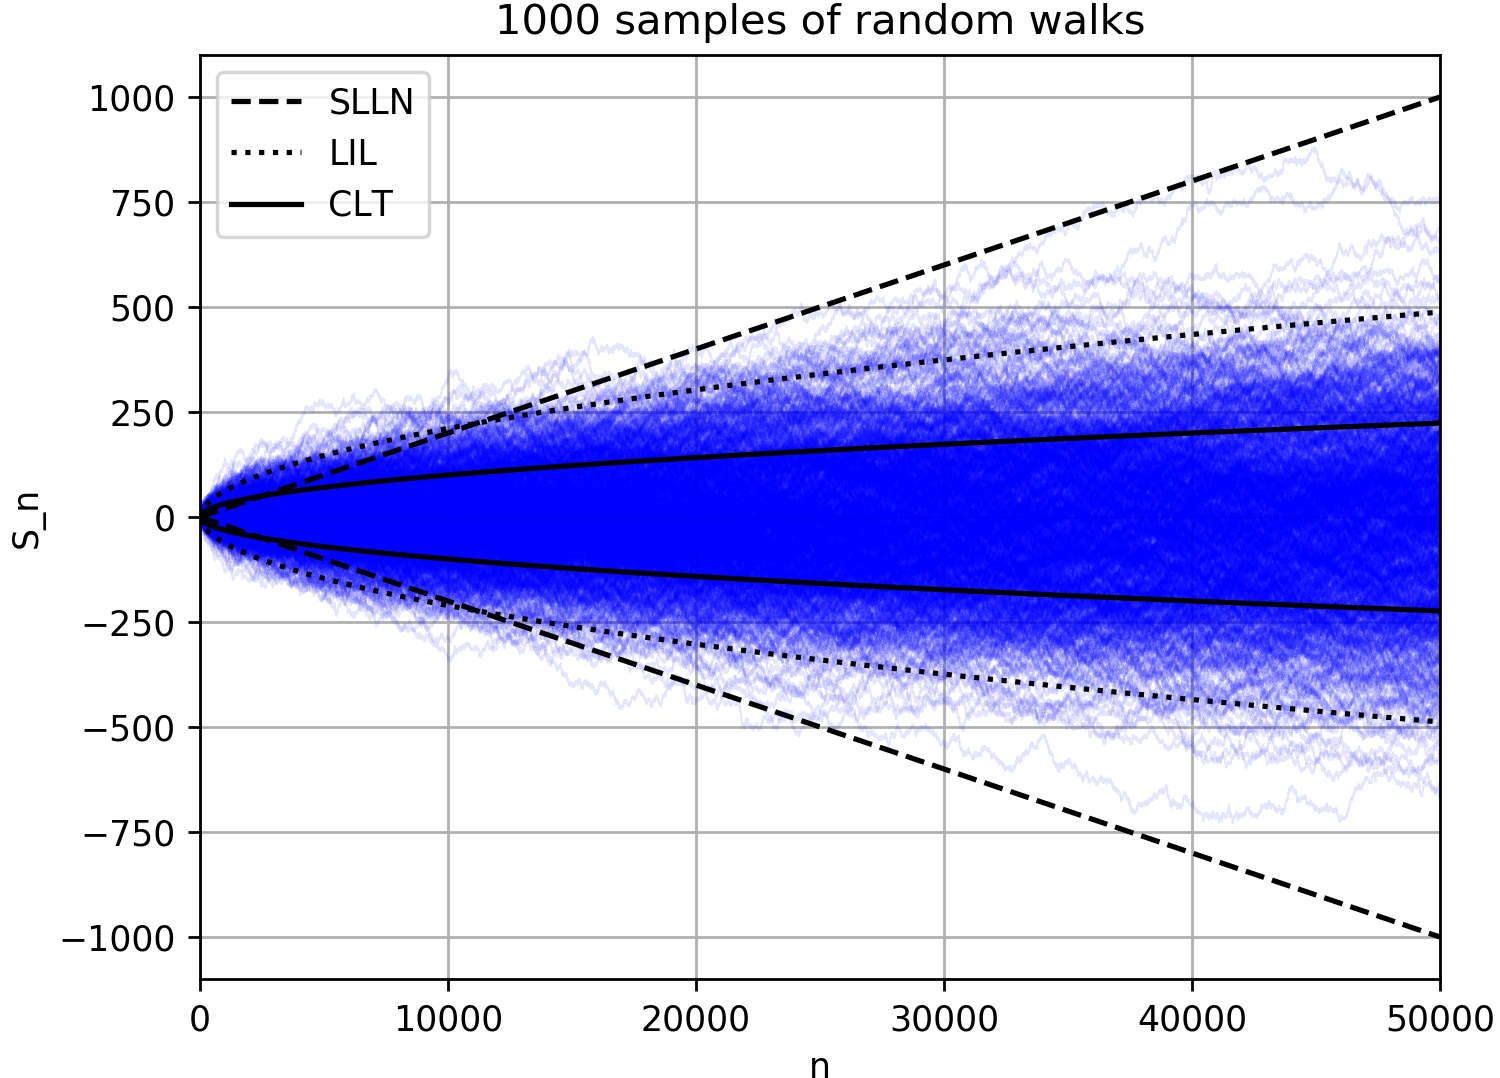
\includegraphics[width=\linewidth]{1000_random_walks}
	\caption{$1000$ samples of random walks, with each step having mean $0$ and variance $1$. Almost all the walks eventually fall inside the outer dashed cone of $y = \pm \epsilon n$, demonstrating the SLLN. Most of the walks barely touch the edges of the cone $y = \pm \sqrt{2 n \ln\ln{n}}$, demonstrating the LIL. About 68\% of the walks are inside the cone $y = \pm \sqrt{n }$ at the right edge of the graph, demonstrating one instance of the CLT.}
	\label{fig:lil}
\end{figure}

SLLN states that for any $\epsilon > 0$, with probability one, a randomly chosen walk would eventually be contained in the cone $y = \pm \epsilon x$.

CLT states that for any $\epsilon > 0$, for big $n$, the probability that a randomly chosen path is within the cone $y = \pm \epsilon \sqrt{x}$ at the $x = n$ section (that is, $S_n \in (-\epsilon \sqrt{x}, \epsilon \sqrt{x})$) is $Pr(\mathcal{N}(0, 1)\in (-\epsilon, \epsilon))$.

Intermediately, LIL states that with probability one, a random path would touch the edge of the cone $y = \pm \sqrt{2 x \ln\ln{x}}$ infinitely many times, but for any $\epsilon > 0$, it would only touch the edge of $y = \pm (1+\epsilon )\sqrt{2 x \ln\ln{x}}$ finitely many times.

While SLLN and CLT are extensively used in practical statistics, the LIL in comparison has little practical consequence \cite{vandervaartAsymptoticStatistics2000}. One classic paper on applications of LIL to statistics is \cite{robbinsStatisticalMethodsRelated1970}.

Before plunging into large deviation theory, which we will use to derive the CLT for certain risk measures, we take note of the surrounding territory for context.

In the literature, one can often find mentions of \textbf{large/moderate/small deviation principles}. Among these, the \textit{large} deviation principles are the most popular. Two standard references on this subject are \cite{demboLargeDeviationsTechniques2009, denhollanderLargeDeviations2008}.

\subsection{Deviation principles}
Consider a random variable $X$ with mean $0$ and variance $1$, and its IID process $(X_n)_n$. Let $S_n = X_1 + \cdots + X_n$. By the CLT, we have for any constant $\epsilon > 0$, 
\begin{equation}
\lim_n Pr(S_n > \epsilon n^{\frac 1 2}) = 1 - \Phi(\epsilon),
\end{equation}
where $\Phi$ is the CDF of the standard normal distribution.

If $|X|$ has finite third moment, then by the Berry--Esseen theorem \cite[Theorem 3.4.9]{durrettProbabilityTheoryExamples2010}, this convergence is uniform in the sense that 
\begin{equation}
\lim_n \frac {Pr(S_n > x_n n^{\frac 1 2})}  {1 - \Phi(x_n)} = 1
\end{equation}
for any sequence of $(x_n)_n$ that satisfies $x_n = O(1)$. This, though not often called so, is a \textit{small} deviation principle.

One immediately considers generalization for $x_n$ that may grow faster than $O(1)$. 

The large deviation theorem would give an asymptotic expansion in the case where $x_n$ is $O(n^{\frac 1 2})$. For example, Cram\'er's theorem states that if $X$ is "nice", there exists a \textbf{rate function} $I : \mathbb{R} \to [0, \infty)$ such that 

$$\forall \epsilon > 0, \: 
Pr(S_n > \epsilon n) \to e^{-nI(\epsilon)}.$$

More rigorously, the convergence is 
\begin{equation}
\frac 1 n \ln Pr(S_n > \epsilon n) \to -I(\epsilon).
\end{equation}

Between them, a moderate deviation theorem \cite{chenSteinIdentitiesModerate2013} states that the asymptotic expansion is
\begin{equation}
	\frac {Pr(S_n > x_n n^{\frac 1 2})}  {1 - \Phi(x_n)} = 1 + O(1) \frac{1 + x^3_n}{\sqrt{n}}.
\end{equation}
for $x_n = O(n^{\frac 1 6})$. In more details, it states that 
\begin{equation}
	\left(\frac {Pr(S_n > x_n n^{\frac 1 2})}  {1 - \Phi(x_n)} - 1\right) \frac{\sqrt{n}}{1 + x^3_n}.
\end{equation}
is bounded as $n\to\infty$.

In \cite{rubinProbabilitiesModerateDeviations1965}, a moderate deviation defined by $x_n = O(\sqrt{\ln{n}})$ is studied. In general, moderate deviation studies 
$$O(1) < x_n < O(\sqrt{n}),$$
that is, 
\begin{equation}
|x_n| \to \infty, \: \frac{x_n}{\sqrt{n}} \to 0.
\end{equation}

A large part of modern probability consists of various generalizations of the deviation principles under assumptions on $(X_n)_n$ weaker than full independence
\footnote{Such as "weakly dependent", "strongly mixing", "exchangeable", "ergodic", and many other highly technical weakenings.}. The sequences of $(X_n)_n$ could also be generalized to be multidimensional, or graphs, or some other complicated mathematical objects.

\subsection{The G\"artner--Ellis theorem}
The G\"artner--Ellis theorem states a large deviation principle for sequences of not necessarily independent random variables. It uses a generalization of the cumulant generating function:

\begin{defn}
For any real random variable $X$, its \textbf{cumulant generating function} is
\begin{equation}
\forall t\in \mathbb{R}, \quad K(t) = \ln\mathbb{E}(e^{tX}).
\end{equation}
\end{defn}


Consider, for example, the empirical process $(L_n)$ of $X$, and the sequence $\mathbb{E}(L_n) = \frac 1 n \sum_{i=1}^n X_i$, then we have 
$${\mathbb{{{E}}}}{\left({e}^{{{n}{t}{\mathbb{{{E}}}}{\left({L}_{{n}}\right)}}}\right)} = {\mathbb{{{E}}}}{\left({e}^{{{t}{X}}}\right)}^{n}
$$
and so for any $t\in\mathbb{R}$,
$$K(t) = \lim_{n\to \infty}\frac 1 n \ln {\mathbb{{{E}}}}{\left({e}^{{{n}{t}{\mathbb{{{E}}}}{\left({L}_{{n}}\right)}}}\right)}$$

For a general sequence of real random variables, $(Y_n)_n$, let 
$$K_n(t) = \frac 1 n \ln {\mathbb{{{E}}}}{\left({e}^{{{n}{t}{\mathbb{{{E}}}}{\left({L}_{{n}}\right)}}}\right)},$$
then if the following limit exists
$$\lim_{n\to \infty}K_n(t)$$
for all $t$ in a neighborhood of $0$, then the G\"artner--Ellis theorem gives the limit behavior of a properly scaled version of the sequence $(Y_n)_n$.

There are many versions of the G\"artner--Ellis theorem with varying generalities. The version that we use is \cite[Lemma 1]{coxLargeDeviationsPoisson1984}:
\begin{theorem}[G\"artner--Ellis theorem]
\label{theorem:gartner}
For a general sequence of real random variables, $(Y_n)_n$, if the following limit exists
$$K(t) = \lim_{n\to \infty}\frac 1 n \ln \displaystyle{\mathbb{{{E}}}}{\left({e}^{{{n}{t}{Y}_{{n}}}}\right)}$$
for $t$ in a neighborhood $(\epsilon_-, \epsilon_+)$ of $0$, and if $K$ is strictly convex and $C^2$ on $(\epsilon_-, \epsilon_+)$, then, letting $\mu = K'(0), \sigma^2 = K''(0)$,
\begin{enumerate}[(1)]
	\item (SLLN) $Y_n \asconv \mu$.
	\item (CLT) If for all sufficiently large $n$, $K_n$ is convex on $[0, \epsilon_+)$, and $\lim_n K_n''(0) = \sigma^2$, then \begin{equation}
		\frac{Y_n - \mathbb{E}(Y_n)}{\sqrt{n}} \distconv \mathcal{N}(0, \sigma^2).
	\end{equation}
%	\item (LDP) Let $\mu_+ = K'(\epsilon_+), \mu_- = K'(\epsilon_-)$, then for all $\zeta\in(\mu, \mu_+)$, \begin{equation}
%		\lim_n \frac 1 n \ln Pr\left(\frac{Y_n}{n} > \zeta\right) = -K^*(\zeta)
%	\end{equation}
%	and similarly for all $\zeta\in(\mu_-, \mu)$, \begin{equation}
%	\lim_n \frac 1 n \ln Pr\left(\frac{Y_n}{n} < \zeta\right) = -K^*(\zeta)
%	\end{equation}
\end{enumerate}
\end{theorem}

\section{Limit theorems of \cvar}
In this section, we present calculations and numerical evidence that demonstrate, if not prove with full rigor, the CLT and SLLN of \cvar.

\subsection{CLT for \cvar}
\label{sec:clt_cvar}

Consider a real $X$ with PDF $\rho$ and CDF $\Phi$. For any $h \in \mathbb{N}$, define 
\begin{align*}
\label{eq:temp_1}
\mathbb{E}(\exp{(nt \cvar_\alpha(L_n))}) &= \mathbb{E}\left(\exp{\left( \frac{t}{\overbar{\alpha}} \sum_{i=1}^{\overbar{\alpha} n} X_{(i)} \right)}\right) \\
&= \mathbb{E}\left(\exp{\left( \frac{t}{\overbar{\alpha}} \sum_{i=1}^{\overbar{\alpha} n} X_i \right)} \Big| X_1, ..., X_{\overbar{\alpha} n} > X_{\overbar{\alpha} n + 1} > X_{\overbar{\alpha} n + 2} , ... X_n\right) 
\end{align*}
Here, $X_{(i)}$ denotes the i-th biggest term in the sequence $X_1, ... X_n$. The cases where two or more $X_i$ are equal having measure $0$, thus ignored.

Note that the sum should not be taken literally, as in actuality, $\cvar_\alpha(L_n)$ is the average of the biggest $\floor{\overbar{\alpha} n}$ terms of $X_1, ..., X_n$, plus $\{\overbar{\alpha} n\}$ times the next biggest term. However, as $n$ grows, this little fudge factor will be swamped out, and therefore we ignore it.

That the expectation can be conditioned on a particular choice of ordering of $X_i$ is because the sequence $(X_n)_n$ is an \textbf{exchangeable sequence of random variables}, that is, any finite permutation of the sequence creates a sequence with the same distribution.

Now we continue the calculation.
\begin{align*}
&= \int_{\mathbb{R}} Pr(X_{\overbar{\alpha} n + 1}\in dx |  X_1, ..., X_{\overbar{\alpha} n} > X_{\overbar{\alpha} n + 1} > X_{\overbar{\alpha} n + 2} , ... X_n) \mathbb{E}(e^{\frac{tX}{\overbar{\alpha}}} | X > x)^{\overbar{\alpha} n} \\
&= \int_{\mathbb{R}} 
\frac{F_X(x)^{\alpha n - 1}(1-F_X(x))^{\overbar{\alpha} n} \rho(x) dx}{B(\alpha n, \overbar{\alpha} n + 1)}
\mathbb{E}(e^{\frac{tX}{\overbar{\alpha}}} | X > x)^{\overbar{\alpha} n}
\end{align*}
where $B(x, y) = \frac{\Gamma(x)\Gamma(y)}{\Gamma(x+y)}$ is the Euler beta function, and $\Gamma$ is the Euler gamma function.

Plugging in 
$$(1-F_X(x))\mathbb{E}(e^{\frac{tX}{\overbar{\alpha}}} | X > x) = \int_x^\infty  e^{ty/\overbar{\alpha}} \rho(y)dy, $$
we obtain
\begin{align*}
&= \frac{1}{B(\alpha n, \overbar{\alpha} n + 1)}\int_{\mathbb{R}} 
\left(F_X(x)^\alpha \left(\int_x^\infty  e^{ty/\overbar{\alpha}} \rho(y)dy\right)^{\overbar{\alpha}}\right)^n
\frac{\rho(x)}{F_X(x)}dx
\end{align*}

Now, by Stirling's approximation, 
$$B(\alpha n, \overbar{\alpha} n + 1) = \exp(-n H(\alpha) + O(\ln n)),$$
where 
\begin{equation}
H(\alpha) = -\alpha \ln \alpha - \overbar{\alpha} \ln \overbar{\alpha}
\end{equation} 
is the binary entropy function.

So, by Laplace's method 
\cite[Section 6.4]{benderAdvancedMathematicalMethods1999}, 
\begin{equation}
K(t) = H(\alpha) + \max_{x\in\mathbb{R}}
\left(\alpha \ln F_X(x)
+
\overbar{\alpha}\ln\left(\int_x^\infty  e^{ty/\overbar{\alpha}} \rho(y)dy\right)\right)
\end{equation}
provided that 
\begin{equation}
	\label{eq:maxfun}
\alpha \ln F_X(x)
+
\overbar{\alpha}\ln\left(\int_x^\infty  e^{ty/\overbar{\alpha}} \rho(y)dy\right)
\end{equation}

has a unique global maximum at some $x_0$, is $C^2$ in a neighborhood of $x_0$, and $\frac{\rho(x_0)}{F_X(x_0)}> 0$. 

Taking derivative, such a maximum is a root of 
\begin{equation}
\label{eq:maxfun_root}
F_X(x) = \frac{\alpha}{\overbar{\alpha}}\int_0^\infty e^{ty/\overbar{\alpha}}\rho(x+y)dy.
\end{equation}
At $ t = 0$ has solution $x = F_X^{-1}(\alpha)$, and we obtain
$$K(0) = H(\alpha) + \alpha \ln F_X(F_X^{-1}(\alpha)) + \overbar\alpha\ln\int_{F_X^{-1}(\alpha)}^\infty \rho(y)dy = 0$$
as it should.

Near $t=0$, $x$ can be expanded as a power series $x = F_X^{-1}(\alpha) + x_1 t + x_2 t^2 + o(t^2) $, which can then be plugged into the equation of $K(t) = \mu(\alpha) t + \frac 12 \sigma(\alpha)^2 + o(t^2)$, from which we obtain 
\begin{equation}
\sqrt{n}(\cvar_\alpha(L_n) - \mu(\alpha))\distconv \mathcal{N}(0, \sigma(\alpha)^2)
\end{equation}

\begin{ex}
$X$ is uniform on $[0, 1]$, then
\begin{equation}
K(t) = H(\alpha) + \max_{x\in(0, 1)}
\left(\alpha \ln x
+
\overbar{\alpha}\ln\frac{\overbar{\alpha}}{t}\left(e^{t/\overbar{\alpha}} - e^{tx/\overbar{\alpha}}\right)\right)
\end{equation}

The maximizer $x$ is the root of 
$$x = \frac{\alpha}{t}\left(e^{t(1-x)/{\overbar\alpha}} - 1\right)$$
which has asymptotic expansion 
$$x = \alpha + x_1 t + x_2 t^2 + o(t^2).$$
Plugging it in and solving up to $t^2$ order, we obtain 
$$ x = \alpha + \frac 12 \alpha{\overbar\alpha} t + \frac 16 \alpha{\overbar\alpha}(1-3\alpha) t^2 $$
and so 
$$K(t) = \frac 12 (1+\alpha) t + \frac{1}{24}(1-\alpha)(1+3\alpha)t^2 + o(t^2)$$
So we obtain the CLT for $X$:
\begin{equation}
\label{eq:uniform_std}
\mu(\alpha) = \frac 12 (\alpha+1) = \cvar_\alpha(X), \quad \sigma(\alpha)^2 = \frac{1}{12}(1-\alpha)(1+3\alpha)
\end{equation}

This is illustrated in Figures \ref{fig:cvar_uniform_clt} and \ref{fig:cvar_stds}.
\end{ex}

\begin{figure}
	\centering
	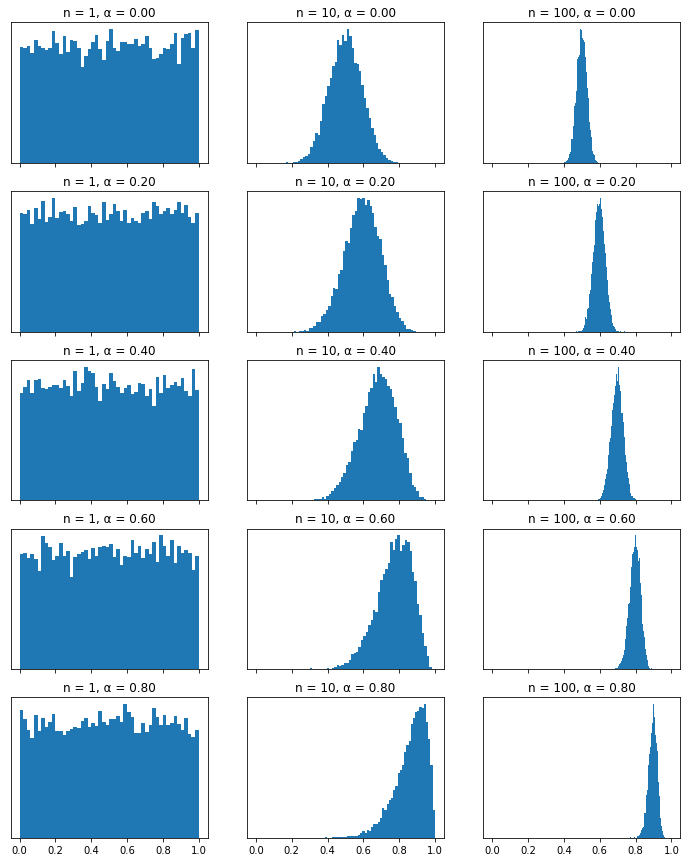
\includegraphics[width=0.9\textwidth]{cvar_uniform_clt.png}
	\caption{A demonstration of the CLT for \cvar. Here, $X$ is the uniform distribution on $[0, 1]$, and the PDF of $\cvar_\alpha (L_n)$ is plotted as a function of $n$ and $\alpha$. As $n$ increases, the distributions converge to normal distributions. Increasing $\alpha$ both shifts the distribution to the right, and distort it away from normality. Each histogram is the result of $10^4$ trials.}
	\label{fig:cvar_uniform_clt}
\end{figure}

\begin{figure}
	\centering
	\begin{subfigure}[b]{0.45\textwidth}
		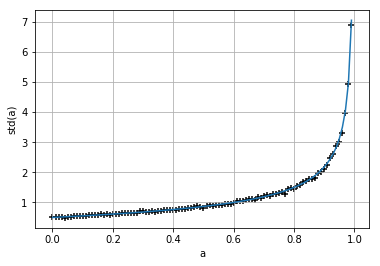
\includegraphics[width=\textwidth]{exponential_std.png}
		\caption{$\rho(x) = 2e^{-2x}$ with $x > 0$.}
		\label{fig:exp_std}
	\end{subfigure}
	~
	\begin{subfigure}[b]{0.45\textwidth}
		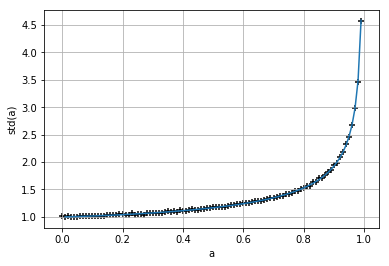
\includegraphics[width=\textwidth]{gaussian_std.png}
		\caption{$X\sim \mathcal{N}(0, 1)$.}
		\label{fig:gaussian_std}
	\end{subfigure}
	~
	\begin{subfigure}[b]{0.45\textwidth}
		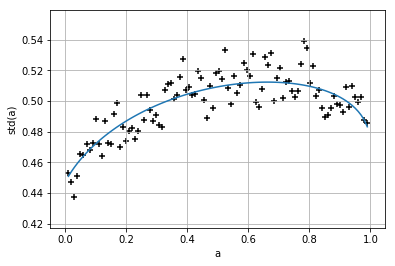
\includegraphics[width=\textwidth]{parabolic_std.png}
		\caption{$\rho(x) = \frac 34 (1-x^2)$ with $x\in[-1, 1]$}
		\label{fig:parabolic_std}
	\end{subfigure}
	~
	\begin{subfigure}[b]{0.45\textwidth}
		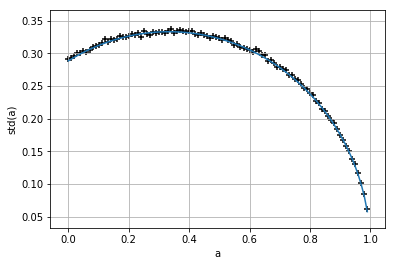
\includegraphics[width=\textwidth]{uniform_std.png}
		\caption{$X$ is uniform on $[0, 1]$.}
		\label{fig:uniform_std}
	\end{subfigure}
	~
	\begin{subfigure}[b]{0.45\textwidth}
		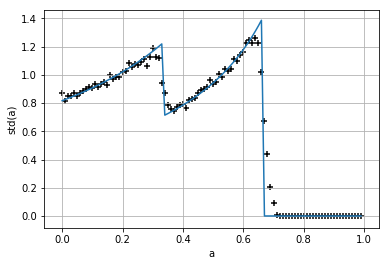
\includegraphics[width=\textwidth]{discrete_0_1_2_std.png}
		\caption{$X$ is discrete uniform on $\{0, 1, 2\}$.}
		\label{fig:discrete_0_1_2_std}
	\end{subfigure}
	~
	\begin{subfigure}[b]{0.47\textwidth}
		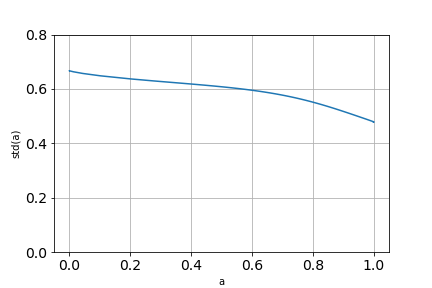
\includegraphics[width=\textwidth]{xex2_std.png}
		\caption{$\rho(x) = -xe^{-x^2/2}$ with $x< 0$.}
		\label{fig:xex2_std}
	\end{subfigure}
	\caption{Numerical confirmation of Theorem \ref{theorem:clt_cvar} (CLT for \cvar). $\sigma(\alpha)$ plots for six different distributions of $X$ are calculated, and five of them fits the numerical simulation. The last plot is calculated only theoretically, without numerical verification. The curves are the exact theoretical prediction of the standard deviation of $\sqrt{n}\cvar_\alpha(L_{n})$ as $n\to \infty$, given by Equation \ref{eq:clt_cvar}. Each point in the scatterplots is obtained by sampling $\sqrt{n}\cvar_\alpha(L_{n})$ for $1000$ times, where $n = 1000$. }
	\label{fig:cvar_stds}
\end{figure}

\begin{ex}
A discrete $X$ with a finite discrete distribution $\sum_{i = 1}^N p_i \delta_{x_i}$ can be approximated by very concentrated uniform distributions, that is, 
$$\rho(x) = \begin{cases}
\frac{p_i}{\epsilon}\quad x\in[x_i, x_i+\epsilon]\\
0 \quad \text{else}
\end{cases}, 
$$
where $\epsilon$ is a positive number smaller than $\min_{1 \le i \le N-1}(x_{i+1} - x_i)$.

Let $P_i = p_1 + ... + p_i$ for all $i\in [N]$, then if $\alpha \in (P_{i-1}, P_i)$ for some $i\in [N]$, then $F_X^{-1}(\alpha) =x_i + \frac{\epsilon}{p_i} (\alpha - P_{i-1})$. Then, the maximum in Equation \ref{eq:maxfun} is the root of 
$$P_{i-1} + \frac{p_i}{\epsilon}(x-x_i) = \frac{\alpha}{\epsilon t}
\left(p_i \left(e^{(\epsilon - (x-x_i))t/{\overbar\alpha}} - 1\right) + 
\sum_{j = i+1}^N \left(p_j e^{(x_j - x)t/{\overbar\alpha}} \left(e^{\epsilon t/{\overbar\alpha}} - 1\right) \right)\right)$$
which has the power expansion
$$ x =  x_i + \frac{\epsilon}{p_i} (\alpha - P_{i-1}) + A t + Bt^2 + o(t^2)$$

Plugging it in to solve for $A, B$, then expanding $K$, and taking the $\epsilon \to 0$ limit, we obtain 
$$K(t) = \mu(\alpha) t + \frac 12 \sigma(\alpha)^2 t^2$$ 
where
\begin{equation}
\mu(\alpha) = \frac{1}{{\overbar\alpha}}( x_i (P_i - \alpha) + \sum_{k > i}^N p_k x_k) = \cvar_\alpha(X), 
\end{equation}
\begin{equation}
\sigma(\alpha)^2 = \frac{1}{{\overbar\alpha}^2} \left((P_i(1-P_i)x_i^2 - 2P_ix_i \sum_{k > i}^N p_k x_k + \sum_{k > i}^N p_k x_k^2 - \left(\sum_{k > i}^N p_k x_k\right)^2\right)
\end{equation}

After routine algebra, this is simplified to $\mathbb{V}\left(\frac 1{\overbar\alpha} (X - F_X^{-1}(\alpha))^+\right)$, where for any random variable $Y$, $Y_+ = \max(Y, 0)$ is the positive part of $Y$.
\end{ex}

When $\alpha$ is equal to some $P_i$, that is, when $F_X^{-1}$ is discontinuous at $\alpha$, the result is not determined by this method, as $K(t)$ does not have continuous second-derivative in a neighborhood of $t = 0$. 

For arbitrary $X$ with finite variance, its distribution can be approximated as the limit of discrete distributions, and so we have obtained
\begin{theorem}[CLT for \cvar]
\label{theorem:clt_cvar}
For any real random variable $X$ with finite variance, and any $\alpha\in(0, 1)$, if $F_X^{-1}$ is continuous  at $\alpha$, then the empirical process of the $\cvar_\alpha$ of $X$ satisfies
\begin{equation}
\label{eq:clt_cvar_distconv}
\sqrt{n}(\cvar_\alpha(L_n) - \cvar_\alpha(X)) \distconv \mathcal{N}\left(0, \sigma(\alpha)\right)
\end{equation}
where 
\begin{align}
\begin{split}
\label{eq:clt_cvar}
\sigma(\alpha)^2
 &= \frac 1{\overbar\alpha} \mathbb{E}[(X- F_X^{-1}(\alpha))^2|X > F_X^{-1}(\alpha)] 
   -  \mathbb{E}[(X- F_X^{-1}(\alpha)) | X > F_X^{-1}(\alpha)]^2\\
 &= \mathbb{V}\left(\frac 1 {\overbar\alpha} (X - F_X^{-1}(\alpha))^+\right)
\end{split}
\end{align}


\end{theorem}

A more abstract and general version of the CLT for empirical \cvar, that weakens assumption of independence of the process $(X_n)$ to merely $\alpha$-mixing, is proved in \cite[Theorem 1]{chenNonparametricEstimationExpected2007}.

In \cite[Theorem 3.1]{brazauskasEstimatingConditionalTail2008}, an alternative formula for $\sigma(\alpha)$ is given:
\begin{equation}
\label{eq:alt_cvar_std}
\sigma(\alpha)^2=\frac{1}{(1-\alpha)^{2}} \int_{F_{X}^{-1}(\alpha)}^{\infty} \int_{F_{X}^{-1}(\alpha)}^{\infty}\left(F_{X}(\min(x, y))-F_{X}(x) F_{X}(y)\right)dx dy
\end{equation}

As for $\alpha$ where $F_X^{-1}$ is discontinuous, we conjecture that the CLT simply fails, and instead, the limit distribution is a "mixed" normal distribution. 

\begin{defn}
	\label{defn:mixed_normal}
	Given $\sigma_1, \sigma_2 > 0$, the mixed normal distribution $\mathcal{N}_{mixed}(\mu, \sigma_1, \sigma_2)$ is the distribution with PDF
	\begin{equation}
	\rho(x) = \begin{cases}
	\rho_1(x) \frac{2 \sigma_1}{\sigma_1 + \sigma_2} \quad x\le \mu \\
	\rho_2(x) \frac{2 \sigma_2}{\sigma_1 + \sigma_2}  \quad x \ge \mu
	\end{cases}
	\end{equation}
	where $\rho_i$ is the PDF of $\mathcal{N}(\mu, \sigma_i)$, with $i = 1, 2$.
\end{defn}

\begin{conj}
	\label{conj:mixed_gaussian}
	Given $X$ with finite variance, for any $\alpha \in(0, 1)$ such that $F_X^{-1}$ is discontinuous at $\alpha$,  
	
	\begin{equation}
	\sqrt{n}(\cvar_\alpha(L_n) - \cvar_\alpha(X)) \distconv \mathcal{N}_{mixed}(\mu, \sigma_1, \sigma_2)
	\end{equation}
	where 
	\begin{equation}
	\mu = \cvar_\alpha(X),
	\end{equation}
	and 
	\begin{equation}
	\sigma_1 = \lim_{z \nearrow \alpha}\sigma(z), \quad
	\sigma_2 = \lim_{z \searrow \alpha}\sigma(z).
	\end{equation}
	are the two one-sided limits of $\sigma(\alpha)$.
\end{conj}


This conjecture cannot be proved by Theorem \ref{theorem:gartner}, since when $\alpha$ is at those critical values, $K(t)$ has no second-derivative at $0$.

We tested this conjecture by numerically calculating the distribution of\\ $\cvar_\alpha(L_n)$, for a big $n = 10^5$, $X$ being uniformly distributed on $\{0, 1, 2\}$, and for $\alpha\approx 1/3$, around a discontinuous point of $F_X^{-1}$. 

As shown in Figure \ref{fig:cvar_boundary_behavior_discrete_0_1_2_shifting}, as $\alpha$ is about the discontinuous point, the right side of the bell curve suddenly shrinks in width from $\sigma_l$ down to $\sigma_u$. Then, just after $\alpha$ crosses the discontinuity, left side shrinks too.

The conjecture predicts that it should have a mixed normal distribution defined by 
$$\mu = 1.5, \sigma_l = \sqrt{1.5/n} = 0.003873 , \sigma_u = \sqrt{0.5/n} = 0.002236.$$

As shown in Figure \ref{fig:cvar_boundary_behavior_discrete_0_1_2}, this is close to the numerical best fit
$$\mu = 1.5 + 2.1\times 10^{-4}, \sigma_l = 0.003729, \sigma_u = 0.002217.$$

\begin{figure}
	\centering
	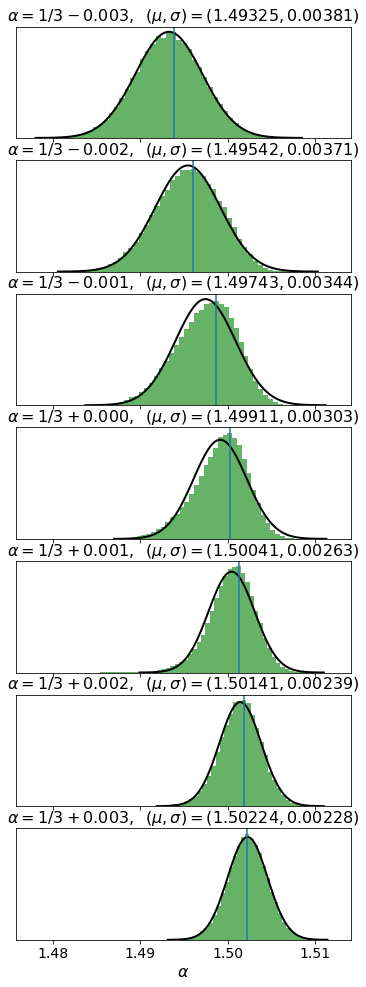
\includegraphics[width=0.5\textwidth]{cvar_boundary_behavior_discrete_0_1_2_shifting.png}
	\caption{Distribution of $\cvar_{\alpha}(L_n)$, with $n=10^5$, $X$ being the uniform distribution on $\{0, 1, 2\}$, as $\alpha$ crosses the $1/3$ boundary. Each histogram results from $10^5$ trials. Each black curve is the best fit normal distribution $\mathcal{N}(\mu, \sigma)$, with parameters $\mu, \sigma$ written above. Each vertical line denotes the estimated maximum of the distribution of $\cvar_\alpha(L_n)$. Notice how nearing $\alpha=1/3$, the fit to normal distribution degrades , and the estimated maximum shifts ahead.}
	\label{fig:cvar_boundary_behavior_discrete_0_1_2_shifting}
\end{figure}

\begin{figure}
	\centering
	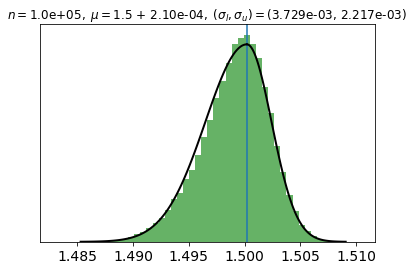
\includegraphics[width=0.6\textwidth]{cvar_boundary_behavior_discrete_0_1_2.png}
	\caption{Distribution of $\cvar_{1/3}(L_n)$, with $n=10^5$, $X$ being the uniform distribution on $\{0, 1, 2\}$. The histogram results from $10^5$ trials. The black curve is the best fit mixed normal distribution $\mathcal{N}(\mu, \sigma_l, \sigma_u)$, with $\mu = 1.5 + 2.1 \times 10^{-4}, \sigma_l = 0.003729, \sigma_u = 0.002217$, and the vertical line denotes the location of $\mu$. }
	\label{fig:cvar_boundary_behavior_discrete_0_1_2}
\end{figure}

\subsection{SLLN for \cvar}
\label{sec:slln_for_cvar}
Now we present the SLLN for the empirical process of \cvar assuming $X$ has finite variance. 

In \cite[Proposition 4.1]{acerbiCoherenceExpectedShortfall2002}, this is proved assuming only that $$\mathbb{E}((-X)^+)<\infty,$$
but the proof is more involved. 

\begin{theorem}[SLLN for \cvar]\label{thm:slln_cvar}
For any real random variable $X$ with finite variance, and any $\alpha\in[0, 1]$, then the empirical process of the $\cvar_\alpha$ of $X$ satisfies
\begin{equation}
\cvar_\alpha(L_n) \asconv \cvar_\alpha(X).
\end{equation}
\end{theorem}

\begin{proof} There are four cases to consider.
	
	1. If $\alpha = 0$, it is simply the SLLN for expectations.
	
	2. If $\alpha = 1$, it is proved in Theorem \ref{theorem:slln_esssup}.
	
	3. If $\alpha\in(0, 1)$, and $F_X^{-1}$ is continuous at $\alpha$, then the power series $K(t) = \mu(\alpha) t + \frac 12 \sigma(\alpha)^2 t^2 + o(t^2)$ in a neighborhood of $0$ means that $K$ is stricly convex and $C^2$ in that neighborhood. Now apply part (a) of Theorem \ref{theorem:gartner}.
	
	4. If $\alpha_0\in(0, 1)$, and $F_X^{-1}$ is not continuous at $\alpha_0$, then we prove by "squeezing with nearby points of continuity". 
	
	Since $F_X^{-1}$ is monotone, by Lebesgue's differentiation theorem \cite[Section 6.2]{roydenRealAnalysis2010}, it is almost everywhere differentiable. That is, let 
	$$D = \{x \in(0, 1): F_X^{-1} \text{ is differentiable at } x\}$$
	then $D$ has Lebesgue measure $1$.
	
	For any $\epsilon > 0$, since $\cvar_\alpha(X)$ is a continuous function of $\alpha$, there exists $\delta > 0$ such that 
	$$\forall\alpha \in(\alpha_0 - \epsilon, \alpha_0  + \epsilon), 
	|\cvar_\alpha(X) - \cvar_{\alpha_0}(X)| < \delta$$
	
	Now take $\alpha_1, \alpha_2 \in D\cap (\alpha_0 - \epsilon, \alpha_0  + \epsilon)$ such that $\alpha_1 < \alpha_0 < \alpha_2$. Note that $\alpha_1, \alpha_2$ exists because $D$ has measure $1$. 
	
	Then, by the SLLN for $\cvar_{\alpha_1}, \cvar_{\alpha_2}$, and the monotonicity of $\cvar_\alpha$ as a function of $\alpha$, we have 
	$$\limsup_n \cvar_{\alpha_0}(L_n) 
	\le \limsup_n \cvar_{\alpha_2}(L_n) \asconv \cvar_{\alpha_2}(X) 
	\le \cvar_{\alpha_0}(X) + \epsilon$$
	and similarly, 
	$$
	\liminf_n \cvar_{\alpha_0}(L_n) 
	\ge \cvar_{\alpha_0}(X) - \epsilon \text{ almost surely}
	$$
	Since for all $\epsilon > 0$, these two inequalities hold almost surely, we have, almost surely,
	$$\lim_n \cvar_{\alpha_0}(L_n) 
	= \cvar_{\alpha_0}(X).$$
\end{proof}

In fact, with a little manipulation, we immediately strengthen it to 
\begin{theorem}[Uniform SLLN for \cvar]
	\label{theorem:uni_slln}
	For any real random variable $X$ with finite variance, almost surely, for any $\alpha\in[0, 1]$, the empirical process of the $\cvar_\alpha$ of $X$ satisfies
	\begin{equation}
	\cvar_\alpha(L_n) \to \cvar_\alpha(X).
	\end{equation}
	that is, 
	\begin{equation}
		Pr\left(\forall \alpha\in[0, 1], \; \cvar_\alpha(L_n) \to \cvar_\alpha(X)\right) = 1
	\end{equation}
\end{theorem}
\begin{proof}
	Since for any particular $\alpha \in[0, 1]$, 
	$$\cvar_\alpha(L_n) \asconv \cvar_\alpha(X)$$
	so with probability one, it holds simultaneously for the countably many rational $\alpha\in[0, 1]$. Then by a "squeezing" argument like in the previous proof, it holds simultaneously for all $\alpha \in[0, 1]$:
	
	For any $\alpha \in (0, 1)$, and any $\epsilon > 0$, by continuity of $\cvar_\alpha$ with respect to $\alpha$, there exists rational $\alpha_1, \alpha_2 \in(0, 1)$, such that $\alpha_1 < \alpha < \alpha_2$, and 
	$$\cvar_{\alpha}(X) -\epsilon < \cvar_{\alpha_1}(X)\le \cvar_{\alpha}(X)\le \cvar_{\alpha_2}(X) < \cvar_{\alpha}(X) + \epsilon$$
	noting that $\cvar_{\alpha}(X)$ must be finite, since $X$ has finite expectation, and $\alpha < 1$. 
	
	Now, if $\cvar_{\alpha_i}(L_n) \to \cvar_{\alpha_i}(X)$ for $i = 1, 2$, then 
	$$\cvar_{\alpha}(X) -\epsilon \le \liminf_n \cvar_{\alpha}(L_n) $$
	$$\cvar_{\alpha}(X) +\epsilon \ge \limsup_n \cvar_{\alpha}(L_n) $$
	Since this holds for all $\epsilon > 0$, we have 
	$$\cvar_\alpha(L_n) \to \cvar_\alpha(X).$$
\end{proof}

\subsection{CLT of $\cvar_\alpha$ in the $\alpha \to 1$ limit}\label{sec:clt_right_tail}
Now we study the qualitative behavior of 
$$\sigma(\alpha)^2 = \mathbb{V}\left(\frac 1{\overbar\alpha} (X - F_X^{-1}(\alpha))^+\right)$$
at the $\alpha \to 1$ limit.

Let 
\begin{equation}
\
f(\alpha) = {\overbar\alpha} \sigma(\alpha) = \sqrt{\mathbb{V}\left( (X - F_X^{-1}(\alpha))^+\right)}
\end{equation}
then $f$ is a monotonically decreasing function of $\alpha \in (0, 1)$. 

At the $\alpha \to 0$ limit, 
$$f(\alpha) \to \sigma(0)^2 = \mathbb{V}(X).$$

The behavior of $f$ at the $\alpha \to 1$ limit depends on the right tail of the distribution of $X$. Qualitatively speaking, the thinner its right tail, the faster it approaches zero. Figure \ref{fig:schematic_cvar_tail} is a schematic plot of the behavior of $f$, for $X$ with tails of various thicknesses. 

The following examples are summarized by Table \ref{table:cvar_tail}.

\begin{table}[ht]
	\caption{The right tail of ${\overbar\alpha}\sigma(\alpha)$ in the $\alpha\to 1$ limit. The right tail of $\rho$ is either the $x\to \infty$ or the $x\to 0$ limit. As the right tail of $\rho$ becomes thinner, the right tail of ${\overbar\alpha}\sigma(\alpha)$ converges to $0$ quicker.}
	\centering
	$\begin{tabu}{|c|c|}
	\hline
	\text{right tail of }\rho&\text{right tail of }{\overbar\alpha}\sigma(\alpha)\\
	\hline
	\frac{1}{x^{3+\epsilon}}&{\overbar\alpha}^{\frac \epsilon 4}\\ 
	\frac{1}{x^{n}}, (n > 3)&{\overbar\alpha}^{\frac{n-3}{2n-2}}\\ 
	\frac{1}{x^{1001}}&{\overbar\alpha}^{0.499}\\ 
	e^{-x}& {\overbar\alpha}^{0.5}\\ 
	e^{-x^2/2}& \frac{\sqrt{{\overbar\alpha}}}{\erfc^{-1}(2{\overbar\alpha})}\\ 
	(-x)^{999}&{\overbar\alpha}^{0.5005}\\
	(-x)^n, (n > -1)&{\overbar\alpha}^{\frac{n+3}{2n+2}}\\ 
	(-x)^1&{\overbar\alpha}\\ 
	(-x)^0&{\overbar\alpha}^{1.5}\\ 
	(-x)^{-1+\epsilon}&{\overbar\alpha}^{\frac{1}{\epsilon}}\\
	\hline
	\end{tabu}$
	
\label{table:cvar_tail}
\end{table}


Now we list some examples, some of which are shown in Figure \ref{fig:cvar_stds}

\begin{ex}
	Suppose $X$ is uniform on $\{0, 1, 2\}$, then
	\begin{equation}
	\sigma(\alpha)^2 = \begin{cases}
		\frac{2}{3{\overbar\alpha}^2}\text{ if } \alpha\in [0, 1/3)\\
		\frac{2}{9{\overbar\alpha}^2} \text{ if } \alpha\in (1/3, 2/3)\\
		0 \text{ if } \alpha\in (2/3, 1)\\
	\end{cases}
	\end{equation}
	as shown in Figure \ref{fig:discrete_0_1_2_std}.
\end{ex}

\begin{ex}
	Suppose $X$ has a right tail of the form 
	$$\rho(x) \approx \frac{A}{x^n}$$
	where $n > 3$ to ensure that $X$ has finite variance, and $A> 0$ is an unspecified constant, then at the $\alpha \to 1$ limit, approximately 
	\begin{equation}
	\sigma(\alpha)^2 \propto \frac{1}{{\overbar\alpha}^2 \left(-\ln{\overbar\alpha}\right)^{n-3}}
	\end{equation}
	giving $f(\alpha) \propto \left(-\ln{\overbar\alpha}\right)^{-(n-3)/2}$ at $\alpha \to 1$ limit.
\end{ex}

\begin{ex}
	The exponential distribution with PDF 
	$$\rho(x) = \lambda e^{-\lambda x}, x > 0, \lambda > 0$$
	has 
	\begin{equation}
		\sigma(\alpha)^2 = \frac{1}{\lambda^2}\frac{1+\alpha}{1-\alpha}
	\end{equation}
	giving $f(\alpha) \propto {\overbar\alpha}^{1/2}$ at the $\alpha \to 1$ limit. See Figure \ref{fig:exp_std}.
\end{ex}

\begin{ex}
	The Gaussian distribution with PDF 
	$$\rho(x) = \frac{1}{\sqrt{2\pi}}e^{- x^2/2}$$
	has 
	\begin{equation}
	\sigma(\alpha)^2 = \frac{1}{{\overbar\alpha}^2}
	\left(
		1 + \alpha \phi(a)^2 
		+ \frac{\rho(\phi(\alpha))}{\overbar\alpha}((1 -2\alpha)\phi(\alpha) - \rho(\phi(\alpha)))
	\right)
	\end{equation}
	where 
	$$\phi(\alpha) = F_X^{-1}(\alpha) = \sqrt{2} \erf^{-1}(2\alpha - 1)$$
	is its quantile function, where $\erf$ is the error function defined by 
	\begin{equation}
		\erf(x) = 1- \frac{2}{\sqrt{\pi}} \int_{x}^{\infty} e^{-t^{2}} dt
	\end{equation}
	
	At the $\alpha \to 1$ limit, this gives 
	\begin{equation}
	f(\alpha) \approx \frac{\sqrt{{\overbar\alpha}}}{\erfc^{-1}(2{\overbar\alpha})}.
	\end{equation}
	Here, $\erfc$ is the complementary error function, defined by 
	\begin{equation}
	\erfc(x) = 1- \erf(x)
	\end{equation}
	 See Figure \ref{fig:gaussian_std}.
\end{ex}

\begin{ex}
	If $X$ is bounded above, shift it so that $\esssup(X) = 0$. Then suppose it has a PDF $\rho$,
	$$\rho(x) \approx A(-x)^n, x \in (-\epsilon, 0)$$
	where $n > -1$, and $A$ being an unspecified positive constant, then at the $\alpha \to 1$ limit, approximately
	\begin{equation}
	f(\alpha)\propto {\overbar\alpha}^{\frac{n+3}{2n+2}} 
	\end{equation}
	Notably, when $n=1$, $f(\alpha)\propto {\overbar\alpha}$, so $\sigma(\alpha) \propto 1$ in fact converges to a positive constant. This is shown in Figure \ref{fig:parabolic_std}. 
	
	When $ n > 1$, $\sigma(\alpha)$ diverges to infinity, and when $-1 < n < 1$, it converges to $0$. For example, when $X$ is uniform, it has $n=1$, and indeed by Equation \ref{eq:uniform_std}, $\lim_{\alpha \to 1}\sigma(\alpha) = 0$.
\end{ex}

\begin{ex}
	A particularly flat $\sigma(\alpha)$ that we found is shown in Figure \ref{fig:xex2_std}, defined by a real random variable with PDF
	$\rho(x) = -xe^{x^2/2}$, with $x < 0$. It gives
	\begin{equation}
	f(\alpha) = 2({\overbar\alpha} + \alpha^2 F(\sqrt{\ln \alpha})^2)
	\end{equation}
	where $F$ is the Dawson F function defined by
	\begin{equation}
	F(x) = e^{-x^2} \int_0^x e^{t^2} dt.
	\end{equation}
\end{ex}

\begin{figure}
	\centering
	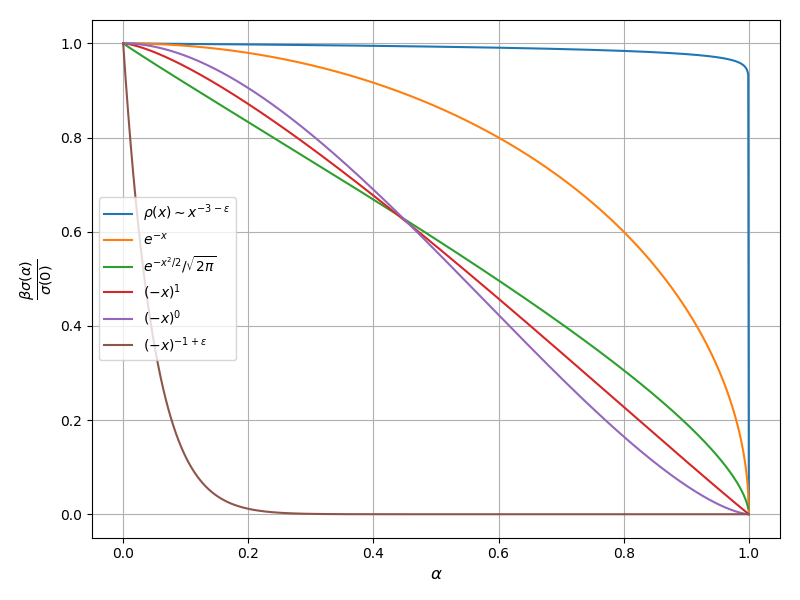
\includegraphics[width=\textwidth]{schematic_cvar_tail.png}
	\caption{Schematic drawing of the tail behavior of ${\overbar\alpha}\sigma(\alpha)$ for various distributions of $X$. In general, the thinner the tail, the faster it converges to $0$.\\
	Each legend lists the right tail of the density the $X$ corresponding to each curve. From top to bottom, the right tails of $X$ and of ${\overbar\alpha}\sigma(\alpha)$ grow thinner together.}
	\label{fig:schematic_cvar_tail}
\end{figure}


\section{Limit theorems for other risk measures}
It is natural to ask whether there are limit theorems for more general risk measures than \cvar. However, a literature search turned up nothing. As such, we believe the following results are new.

\subsection{SLLN for spectral risk measures}
When $X$ is bounded above and below, the uniform SLLN for \cvar can be extended to all spectral risk measures:

\begin{theorem}[uniform SLLN for spectral risk measures]
	\label{thm:uniform_slln_spec}
	Let $X\in \LL^\infty$, that is, it is a random variable with bounded range. Then almost surely, for any probability measure $m$ on $[0, 1]$, the spectral risk measure $\mathcal{F} = \int_0^1 \cvar_\alpha dm(\alpha)$ satisfies a SLLN:
	\begin{equation}
		\mathcal{F}(L_n)\to \mathcal{F}(X)
	\end{equation}
\end{theorem}
\begin{proof}
	Let $M > |X|$ be an upper bound of $X$, then by monotonicity of \cvar, 
	$$-M < \cvar_\alpha(L_n) < M, \; |\cvar_\alpha(L_n)| \le M $$
	By theorem \ref{theorem:uni_slln}, almost surely, $\cvar_\alpha(L_n)$ converges pointwise (with respect to $\alpha$) to $\cvar_\alpha(X)$. Then since $\int M dm(\alpha) = M$ is finite, by Lebesgue's dominated convergence theorem, 
	$$\lim_n\mathcal{F}(L_n) = \lim_n \int \cvar_\alpha(L_n)dm(\alpha) =  \int \cvar_\alpha(X)dm(\alpha) = \mathcal{F}(X)$$
\end{proof}

\subsection{CLT for spectral risk measures?}
In the proof of SLLN for spectral risk measures, the crucial step is using a SLLN of $\cvar_\alpha$ that holds uniformly over all $\alpha\in[0, 1]$. Analogously, we suspect that there is a CLT for spectral risk measures that depends on a uniform CLT, similar to results collected in \cite{dudleyUniformCentralLimit1999}.

In particular, we suspect that a proof can be found through the generalized Berry--Esseen Theorem for \cvar, as \cite[Theorem 1.1]{gaoAsymptoticBehaviorEmpirical2011}:

\begin{theorem}[Berry--Esseen theorem for \cvar]
	Given real random variable $X$ with finite third moment, $\alpha \in (0, 1)$, such that $\sigma(\alpha) > 0$, and $X$ has a strictly positive, continuous PDF in a neighborhood of $F^{-1}(\alpha)$, then there exists some $C_\alpha > 0$ such that
	\begin{equation}
	\|G_n-\Phi\|_\infty \le \frac{C_\alpha}{\sqrt{n}}
	\end{equation} 
	for all $n \in \mathbb{N}$, where $G_n$ is the CDF of the random variable 
	$$\frac{\sqrt n}{\sigma(\alpha)}(\cvar_\alpha(L_n) - \cvar_\alpha(X))$$
\end{theorem}

However, using the Berry--Esseen theorem, we were unable to prove the suspected generalization to the CLT of \cvar, so we leave it as a conjecture:
\begin{conj}[CLT for spectral risk measures]\label{conj:clt_spec}
	For any probability measure $m$ on $[0, 1]$, define a spectral risk measure $\mathcal{F} = \int_0^1 \cvar_\alpha dm(\alpha)$, then for any real random variable $X$ with finite variance, 
	\begin{equation}
	\sqrt{n}(\mathcal{F}(L_n) - \mathcal{F}(X)) \distconv \mathcal{N}(0, \sigma)
	\end{equation}
	for some $\sigma \ge 0$, provided that there does not exist some $\alpha_0\in[0, 1]$, such that $m(\alpha_0) > 0$, and $\sigma(\alpha)$ is discontinuous at $\alpha_0$, where $\sigma(\alpha)$ is the standard deviation of the limit distribution in Equation \ref{eq:clt_cvar_distconv}:
	$$\sqrt{n}(\cvar_\alpha(L_n) - \cvar_\alpha(X)) \distconv \mathcal{N}\left(0, \sigma(\alpha)\right)$$
	
	Otherwise, there exists $\sigma_1 > \sigma_2 \ge 0$ such that 
	\begin{equation}
	\sqrt{n}(\mathcal{F}(L_n) - \mathcal{F}(X)) \distconv \mathcal{N}_{mixed}(0, \sigma_1, \sigma_2)
	\end{equation}
\end{conj}

\subsection{CLT for entropic value at risk?}

Other than \cvar, another example of CRM is the entropic value at risk (\evar), proposed in \cite{ahmadi-javidEntropicValueatriskNew2012}.

\begin{defn}
	\label{defn:evar}
	For any $\alpha \in [0, 1]$, and real random variable $X$, its $\alpha$-level \evar is
	\begin{equation}
	\label{eq:evar_def}
	\evar_\alpha (X) = \inf_{t>0} \frac 1 t \ln\mathbb{E}\left(\frac{1}{1-\alpha}e^{tX}\right)
	\end{equation}
\end{defn}

%The dual representation of \evar is \cite[Theorem 4.9]{ahmadi-javidAnalyticalStudyNorms2017}
%\begin{equation}
%\mathscr{Q}_\alpha = \left\{Z : \mathbb{E} Z=1, Z \geq 0 \text{ and } \mathbb{E} Z \log Z \leq \log \frac{1}{1-\alpha}\right\}
%\end{equation}

The entropic value at risk (\evar) is similar to \cvar, and as such we have reasons to suspect it to have a similar CLT. We attempted to calculate the cumulant generating function for the empirical process of \evar, but without success. 


While having no definitive proof, numerical simulation strongly suggests that there exists a similar CLT for \evar:
\begin{conj}[CLT for EVaR]\label{conj:clt_evar}
Given any $X$ with finite variance, and any $\alpha\in [0, 1)$, its empirical process $L_n$ satisfies
\begin{equation}
	\sqrt{n}(\evar_\alpha(L_n) - \evar_\alpha(X)) \distconv \mathcal{N}(0, \sigma(\alpha))
\end{equation}
where $\sigma(\alpha)$ is a continuous function satisfying $\sigma(0)^2 =\mathbb{V}(X)$. 
\end{conj}

Figure \ref{fig:evar_discrete_0_1_2} plots the mean and standard deviation (normalized by $\sqrt{n}$) of the $\evar_\alpha(L_n)$, while Figure \ref{fig:evar_discrete_0_1_2_clt} shows that as $n\to \infty$, the distribution of $\evar_\alpha(L_n)$ becomes closer to normal distribution.

As shown in Figure \ref{fig:evar_discrete_0_1_2}, numerical calculation does not reveal any discontinuity of $\sigma(\alpha)$, akin to that of \cvar, suggesting that for \evar, the CLT holds for all $\alpha\in[0, 1)$.

\begin{figure}
	\centering
	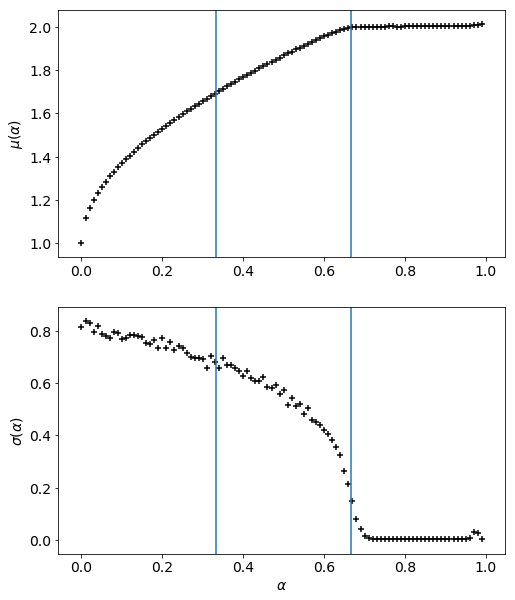
\includegraphics[width=0.7\textwidth]{evar_discrete_0_1_2.png}
	\caption{Mean and standard deviation (normalized by $\sqrt n$) of $\evar_\alpha(L_n)$ plotted as functions of $\alpha$, with $n=1000$, and $X$ being the uniform distribution on $\{0, 1, 2\}$. Each point is calculated from $1000$ trials. The two vertical lines denote $\alpha = 1/3, 2/3$ respectively. As apparent from the graph, $\sigma$ is a continuous function over $[0, 1]$, and equals zero for $\alpha > 2/3$. The blip at the right end of $\sigma(\alpha)$ is due to numerical instability of the root-finding algorithm, which is required in the calculation of $\evar$, as it involves searching for the infimum of a transcendental function, an infimum with no closed form. (see Equation \ref{eq:evar_def}).}
	\label{fig:evar_discrete_0_1_2}
\end{figure}

\begin{figure}
	\centering
	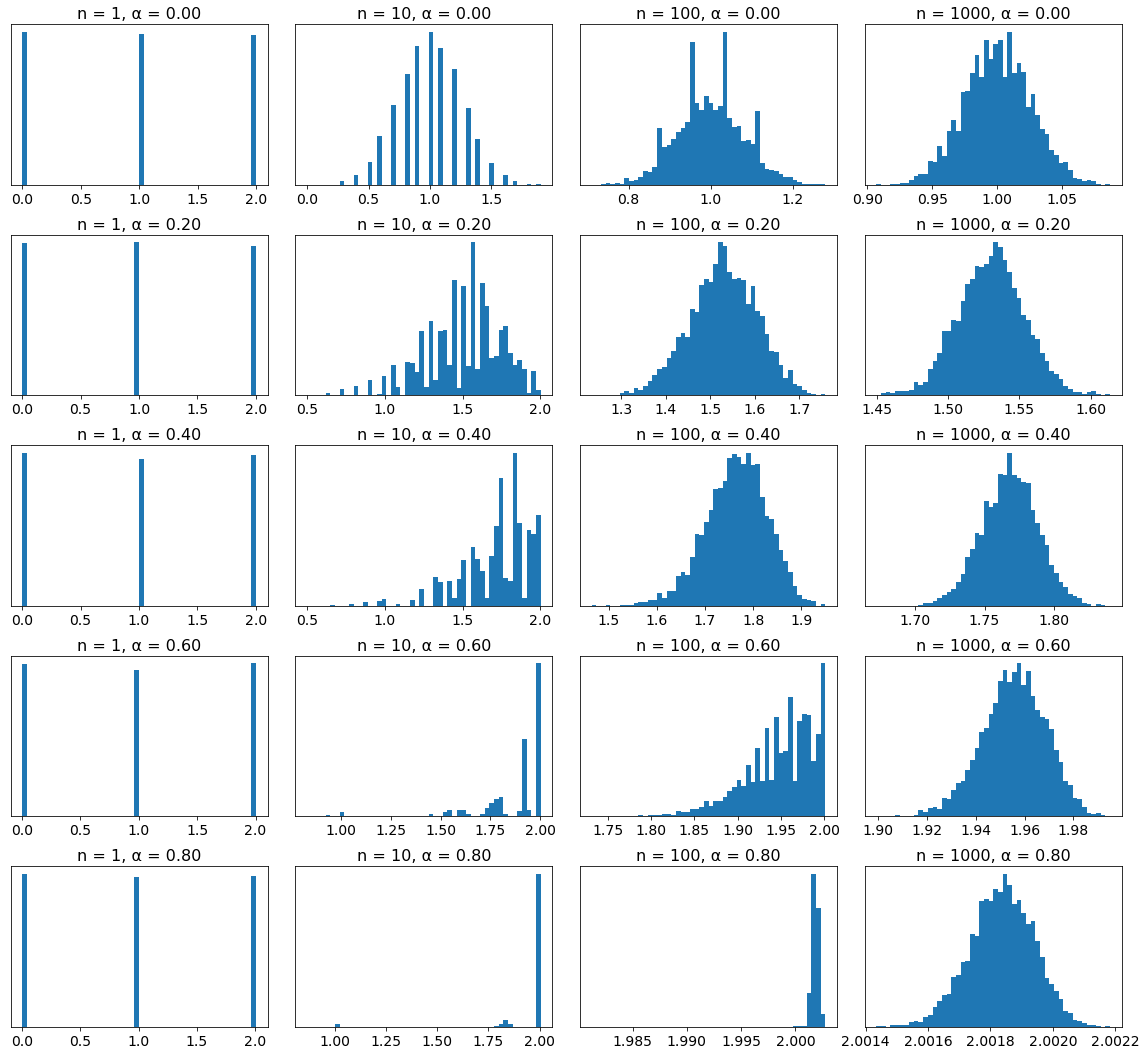
\includegraphics[width=\textwidth]{evar_discrete_0_1_2_clt.png}
	\caption{A demonstration of the CLT for \evar. Here, $X$ is the uniform distribution on $\{0, 1, 2\}$, and the PDF of $\evar_\alpha (L_n)$ plotted as a function of $n$ and $\alpha$. As $n$ increases, the distributions converge to normal distributions. Note that when $\alpha = 0.8$, the distribution becomes close to degenerate, as expected if $\sigma(\alpha) = 0$ when $\alpha > 2/3$. 
	Each histogram is the result of $5000$ trials. The x-axis is shifted and scaled in each plot to make the bell-shape apparent.}
	\label{fig:evar_discrete_0_1_2_clt}
\end{figure}

